\documentclass{article}
\usepackage{graphicx}% Required for inserting images
\usepackage{lindrew}
\usepackage{pdfpages}
\usepackage[shortlabels]{enumitem}
\usepackage{matlab-prettifier}
\usepackage{algorithm}
\usepackage{algpseudocode}

\title{ACM 104 Problem Set 2}
\author{Amitesh Pandey}
\date{October 2024}
\begin{document}
\maketitle
\section*{Problem 1: Subspaces}
(a) We proceed with a proof by counterexample. Let 
\begin{equation*}
    A = \begin{pmatrix}
        0 & 1\\
        0 & 1
    \end{pmatrix}\text{and } B = \begin{pmatrix}
        2 & 0\\
        1& 0
    \end{pmatrix}
\end{equation*}
Then $\det{(A)}, \det{(B)} = 0$ but $\det{(A+B)} = 1 \neq 0$. So $A+B \notin W$, which means $W$ is not closer under addition, so it is not a subspace of $V$. \\\\
\noindent{(b)} (i) See that $\mathbf{0} \in W$ since $\text{tr}\mathbf{0} = 0$. (ii) Now if $A, B \in W$, then
\begin{equation*}
    \sum_{i = 1}^{n}a_{ii} = 0, \sum_{i=1}^{n}b_{ii} = 0 \implies \sum_{i=1}^{n} (a_{ii} + b_{ii}) = 0
\end{equation*}
Then this means $(A+B) \in W$. (iii) Finally also if $A \in W$ then for any $k \in \mathbb{R}$, we have
\begin{equation*}
    \sum_{i=1}^{n} a_{ii} = 0 \implies \sum_{i=1}^{n}ka_{ii} = 0
\end{equation*}
Since $kA \in W$. So $W$ has an identity, is closer under addition, and scalar multiplication, it is a subspace of $V$.  \\\\
\noindent{(c)} We proceed with a proof by counterexample. Let $f_{1}(x) = 1$, then obviously $f_{1}(0)f_{1}(1) = 1$ so $f_{1} \in W$. Then for any $k \in \mathbb{R}$, we have $kf_{1}(x) = k$. So $kf_{1}(0)kf_{1}(1) = k^{2}$. For all $k \in \mathbb{R}\setminus\{-1,1\}$, this condition fails. Since $W$ is not closed under scalar multiplication, it is not a subspace. \\\\
\noindent{(d)} (i) See that if $f(t) = 0$, then
\begin{equation*}
    f\left(\frac{1}{2}\right) = \int_{0}^{1}f(t)\text{d}t = \int_{0}^{1}0\text{d}t = 0
\end{equation*}
so $f(t) = 0 \in W$. (ii) Now if $f_{1}, f_{2} \in W$, then
\begin{equation*}
    (f_{1}+f_{2})(1/2) = \int_{0}^{1}(f_{1}+f_{2})(t)\text{d}t = \int_{0}^{1}f_{1}(t)\text{d}t + \int_{0}^{1}f_{2}(t)\text{d}t = 0 + 0 = 0
\end{equation*}
So $f_{1} + f_{2} \in W$. (iii) Now if $f_{1} \in W$, then
\begin{equation*}
    kf_{1}(1/2) = \int_{0}^{1}kf_{1}(t)\text{d}t = k \int_{0}^{1}f_{1}(t)\text{d}t = k\cdot 0 = 0
\end{equation*}
so $kf_{1} \in W$. $W$ has an identity, is closed under addition and scalar multiplication, so it's a subspace of $V$. \newpage
\noindent{(e)} (i) See that if $v_{z}(x,y)$ such that all points $(x,y)$ map to $\mathbf{0}$, then
\begin{equation*}
    \nabla \cdot v_{z} = \frac{\partial 0}{\partial x} + \frac{\partial 0}{\partial y} = 0 + 0 = 0
\end{equation*}
So $v_{z} \in W$. (ii) Then for $v, v' \in W$, we have
\begin{equation*}
    (v + v')(x,y) = [v_{1}(x,y) + v_{1}'(x,y), v_{2}(x,y) + v_{2}'(x,y)]
\end{equation*}
Then \begin{equation*}
\nabla \cdot (v+v') = \frac{\partial (v_{1} + v_{1}')}{\partial x} + \frac{\partial (v_{2} + v_{2}')}{\partial y} = \frac{\partial v_{1}}{\partial x} + \frac{\partial v_{1}'}{\partial x} + \frac{\partial v_{2}}{\partial y} + \frac{\partial v_{2}'}{\partial y} = 0
\end{equation*}
Thus $(v+v') \in W$. (iii) Now if $v\in W$, then for $kv$, $k \in \mathbb{R}$,
\begin{equation*}
    \nabla \cdot (k v) = \frac{\partial kv_{1}}{\partial x} + \frac{\partial kv_{2}}{\partial y} = k\left(\frac{\partial v_{1}}{\partial x} + \frac{\partial v_{2}}{\partial y}\right) = k(0) = 0
\end{equation*}
So $kv \in W$. $W$ has an identity, is closed under addition and scalar multiplication, so it's a subspace.
\section*{Problem 2: Polynomials}
(a) To check whether the quadratics are linearly independent or not, consider the matrix $A = [p_{1}, p_{2}, p_{3}]$, where $p_{1}, p_{2}, p_{3}$ are the coefficients of the three quadratics. Then
\begin{equation*}
    A = \begin{pmatrix}
        1 & 0 & 1\\
        0 & -1 & 2\\
        -3 & 2 & 1
    \end{pmatrix}
\end{equation*}
Now, if $\text{rank}(A) = 3$, then the quadratics are linearly independent. We know rank is invariant of row operations, so apply the following operations: $r_{3} := r_{3} + 3r_{1}$, and then $r_{3} := r_{3} + 2r_{2}$. Then
\begin{equation*}
    A' = \begin{pmatrix}
        1 & 0 & 1\\
        0 & -1 & 2\\
        0 & 0& 8
    \end{pmatrix}
\end{equation*}
Clearly $A'$ is in row-echelon form and its $\text{rank}(A') = 3$, given by the number of non-zero rows it contains. Since $\text{rank}(A') = 3$, we have also that $\text{rank}(A) = 3$, so the three polynomials are linearly independent. \\\\
(b) Since we have a collection of three polynomials that are linearly independent and all in $\mathcal{P}^{(2)}$, and the fact that any element in $\mathcal{P}^{(2)}$ can be described by a linear combination of three of its linearly independent elements, we can conclude that the three polynomials span $\mathcal{P}^{(2)}$. \\\\
\noindent{(c)} Since $p_{1}, p_{2}, p_{3}$ are linearly independent and span $\mathcal{P}^{(2)}$, we can conclude that they form a basis for it too. It is easy to check that when $q(x) = 1$, we need coordinates $(-1/8, 1/4, 1/8)$ in this basis to achieve $q(x)$.  \newpage
\section*{Problem 3: Fibonacci Sequences}
\noindent{(a)} To show that $\mathcal{F}$ is a vector space, we will first note that $\mathcal{F}$ is a subset of the space of infinitely dimensional real-valued vectors. In other words, $(x_{1},x_{2},\dots x_{n})\in \mathcal{F} \implies (x_{1},x_{2},\dots, x_{n})\in\mathbb{R}^{n}$. Now,
\begin{enumerate}
    \item Identity: When $x_{1}, x_{2} = 0$, $\mathfrak{f}_{z} = (0,0,\dots) \in \mathcal{F}$. So $\mathcal{F}$ has an additive identity.
    \item Closure under addition: Consider $\mathfrak{f}_{1} = (x_{1},x_{2},\dots)$ and $\mathfrak{f}_{2} = (y_{1}, y_{2}, \dots)$, both in $\mathcal{F}$, then by definition we have
    \begin{equation*}
        \mathfrak{f}_{1} + \mathfrak{f}_{2} = \mathfrak{f}_{s} = (x_{1} + y_{1}, x_{2} + y_{2}, \dots)
    \end{equation*}
    Let $\mathfrak{f}_{3} = (z_{1}, z_{2}, \dots)$. For any $k \geq 3$, it is obvious that $z_{k} = x_{k} + y_{k}$. Also, $z_{k - 1} = x_{k-1} + y_{k-1}$ and similarly $z_{k-2} = x_{k-2} + y_{k-2}$. But since $\mathfrak{f}_{1},\mathfrak{f}_{2}\in \mathcal{F}$, we have $x_{k} = x_{k - 1} + x_{k-2}$, and $y_{k} = y_{k-1} + y_{k-2}$. Then
    \begin{equation*}
        z_{k} = x_{k} + y_{k} = x_{k-1} + x_{k-2} + y_{k-1} + y_{k-2} = (x_{k-1} + y_{k-1}) + (x_{k-2} + y_{k-2}) = z_{k-1} + z_{k-2}
    \end{equation*}
    This is sufficient to show that $\mathfrak{f}_{3} = (z_{1},z_{2},\dots)\in \mathcal{F}$
    \item Closure under scalar multiplication: Consider $\alpha \in \mathbb{R}$, and $\mathfrak{f} = (x_{1}, x_{2},\dots) \in \mathcal{F}$, by definintion,
    \begin{equation*}
        \alpha \mathfrak{f} = (z_{1},z_{2}, \dots) = (\alpha x_{1}, \alpha x_{2}, \dots)
    \end{equation*}
    For a $k \geq 3$, we have 
    \begin{equation*}
        z_{k} = \alpha x_{k} = \alpha (x_{k-1} + x_{k-2}) = \alpha x_{k-1} + \alpha x_{k-2} = z_{k-1} + z_{k-2}
    \end{equation*}
    Thus $\alpha \mathfrak{f} \in \mathcal{F}$. So it is closed under scalar multiplication. 
\end{enumerate}
Note that we are permitted to use the distributivity and commutativity of addition because we have already observed that $\mathcal{F}$ is a subset of $\mathbb{R}^{n}$ for arbitrary $n$. Since $\mathcal{F}$ obeys (1), (2), and (3), it is a vector space. \\\\
\noindent{(b)} Note that any generalized Fibonacci sequence only depends on the first two $x_{1},x_{2}$, so $\text{dim}(\mathcal{F}) = 2$. To find $\mathcal{F}$'s basis, we need to find exactly two elements $\mathfrak{f}_{1},\mathfrak{f}_{2} \in \mathcal{F}$ that span $\mathcal{F}$. Note that $\mathfrak{f}_{1} = (1, 0, \dots)$ and $\mathfrak{f}_{2} = (0, 1, \dots)$ are both linearly independent of each other and span $\mathcal{F}$. Thus the basis for $\mathcal{F}$ is $\langle \mathfrak{f}_{1}, \mathfrak{f}_{2}\rangle$. \\\\
\noindent{(c)} It is easy to check that the coordinates of $\mathfrak{f}^{*}$ in that basis are $(1,1)$ since $1\cdot\mathfrak{f}_{1} + 1\cdot\mathfrak{f}_{2} = (1,1, \dots) = \mathfrak{f}^{*}$. 
\newpage
\section*{Problem 4: Fundamental Matrix Subspaces: Low-Dim Example}
(a) Recall that the kernel of $A$, or $\text{Ker}(A)$ is defined as
\begin{equation*}
    \text{Ker}(A) = \{\mathbf{x}\in\mathbb{R}^{2} \ | \ A\mathbf{x} = \mathbf{0}\}
\end{equation*}
\noindent{Essentially}, any $\mathbf{x} = \langle x_{1},x_{2}\rangle \in \text{Ker}(A)$ obeys 
\begin{align*}
    a_{11}x_{1} + a_{12}x_{2} &= 0\\
    a_{21}x_{1} + a_{22}x_{2} &= 0\\
    a_{31}x_{1} + a_{32}x_{2} &= 0
\end{align*}
\noindent{On} substituting from the matrix, we get
\begin{align*}
    2x_{1} + 0x_{2} &= 0\\
    2x_{1} + 2x_{2} &= 0\\
    20x_{1} + 24x_{2} &= 0
\end{align*}
It's easy to see that the solution set to the above equations is unique, thus $\text{Ker}(A) = \{\mathbf{0}\}$, or its $\text{dim}(\text{Ker}(A)) = 0$, since it has no basis. Now for the cokernel of $A$, consider instead the matrix
\begin{equation*}
    A^{T} = \begin{pmatrix}
        2 & 2 & 20\\
        0 & 2 & 24
    \end{pmatrix}
\end{equation*}
Then $\text{coKer}(A) = \text{Ker}(A^{T})$, which is the solution set of
\begin{align*}
    2x_{1} + 2x_{2} + 20x_{3} &= 0\\
    0x_{1} + 2x_{2} + 24x_{3} &= 0
\end{align*}
Which simplifies to $x_{1} = 2x_{3}$, $x_{2} = -12x_{3}$. This can be reduced to the form
\begin{equation*}
    \begin{pmatrix}
        2\\
        -12\\
        1
    \end{pmatrix}
    t = \mathbf{x}
\end{equation*}
Since the vector $\langle 2, -12, 1 \rangle^{T}$ is a basis for $\text{Ker}(A^{T})$, we conclude that $\text{dim}(\text{Ker}(A^{T})) = \text{dim}(\text{coKer}(A)) = 1$. For the image and coimage of $A$, note that the reduced row-echelon form of $A$ is given by
\begin{equation*}
    \text{rref}(A) = \begin{pmatrix}
        1 & 0\\
        0 & 1\\
        0 & 0
    \end{pmatrix}
\end{equation*}
This means that $\text{Im}(A) = \text{span}\{\langle 1, 0, 0 \rangle^{T}, \langle 0, 1, 0\rangle^{T}\}$, since the image is the span of the column vectors and that $\text{coIm}(A) = \text{span}\{\langle 1, 0\rangle, \langle 0, 1\rangle \}$, since it is the span of the non-zero row vectors. This mean that that 
\begin{align*}
    \text{dim}(\text{Im}(A)) &= 2\\
    \text{dim}(\text{coIm}(A)) &= 2
\end{align*}
\noindent{(b)} Since we did not use the rank-nullity theorems for part (a), we have the bases readily available to us in our solution to (a). On compiling the different bases we calculated, we have no basis for $\text{Ker}(A)$, and $\langle 2, 12, 1 \rangle^{T}$ as the basis for $\text{coKer}(A)$, and $\{\langle 1, 0, 0 \rangle^{T}, \langle 0, 1, 0\rangle^{T}\}$ as the basis for $\text{Im}(A)$, and $\{\langle 1,0 \rangle, \langle 0, 1\rangle\}$ as the basis for $\text{coIm}(A)$. 
\section*{Problem 5: Fundamental Matrix Subspaces: High-Dim Example}
Let's proceed with the kernel of $B$. First note that starting at $k = n, n-1, \dots,2$, we can do: $r_{k} := r_{k} - r_{k-1}$. 
\begin{equation*}
    B' = \begin{pmatrix}
        1 & 2 & \dots & n\\
        n & n & \dots & n\\
        \vdots & \vdots & \vdots & \vdots\\
        n & n & \dots & n
    \end{pmatrix} \xrightarrow[\forall k, 3\leq k \leq n]{r_{k} := r_{k} - r_{2}} 
    \begin{pmatrix}
        1 & 2 & \dots & n\\
        n & n & \dots & n\\
        \vdots & \vdots & \vdots & \vdots\\
        0 & 0 & 0 & 0
    \end{pmatrix} \xrightarrow[\forall i, 1\leq i \leq n]{r_{2} := r_{2} - r_{1}}
    \begin{pmatrix}
        1 & 2 & \dots & n\\
        0 & -n & \dots & -n^{2} + n\\
        \vdots & \vdots & \vdots & \vdots\\
        0 & 0 & 0 & 0
    \end{pmatrix}
\end{equation*}
Now we do $r_{2} := r_{2}/(-n)$, to get
\begin{equation*}
    B' = \begin{pmatrix}
        1 & 2 & \dots & n\\
        0 & 1 & \dots& n - 1\\
        \vdots & \vdots & \vdots & \vdots\\
        0 & 0 & 0 & 0
    \end{pmatrix} \xrightarrow{r_{1}:= r_{1} - r_{2}}  \begin{pmatrix}
        1 & 1 & \dots & 1\\
        0 & 1 & \dots& n - 1\\
        \vdots & \vdots & \vdots & \vdots\\
        0 & 0 & 0 & 0
    \end{pmatrix}\xrightarrow{r_{1}:= r_{1} - r_{2}} \begin{pmatrix}
        1 & 0 & \dots & 2-n\\
        0 & 1 & \dots& n - 1\\
        \vdots & \vdots & \vdots & \vdots\\
        0 & 0 & 0 & 0
    \end{pmatrix}
\end{equation*}
This is the reduced row-echelon form of $B$. For $\text{Ker}(B)$, we would have $\mathbf{x}$ such that
\begin{equation*}
    B' \mathbf{x} = 0
\end{equation*}
Let $\mathbf{x} = \langle x_{1}, x_{2}, \dots, x_{n}\rangle$, then
\begin{align*}
    x_{1} + \sum_{i=3}^{n}(2-i)x_{i} &= 0\\
    x_{2} + \sum_{i=3}^{n}(i-1)x_{i} &= 0
\end{align*}
This makes it clear that $x_{1}, x_{2}$ are the pivots and we have $n-2$ free variables $x_{3}, \dots, x_{n}$ such that we only need
\begin{align*}
    x_{1} &= - \sum_{i=3}^{n}(2-i)x_{i}\\
    x_{2} &= - \sum_{i=3}^{n}(i-1)x_{i}
\end{align*}
Now, notice if for each solution $\mathbf{s}_{i} = \langle s_{1}, s_{2}, \dots, s_{n}\rangle$, $3 \leq i \leq n$, we set $s_{i} = 1$ and all other free entries zero, fill $s_{1},s_{2}$ as per the formula above, we will have produced $n-2$ linearly independent vectors in the kernel that span it. Thus the set $S = \{\mathbf{s}_{i} \ | \ 3\leq i \leq n\}$ spans $\text{Ker}(B)$ and forms a basis for it. Since the reduced row-echelon form of $B^{T}$ can be shown to be the same as that of $B$, the basis for the cokernel of $B$ is the same as the basis of the kernel of $B$. Now for the image of $B$, through elementary row operations, we can conclude that the columns $c_{1} = [1, n+1, \dots, n^{2} + n - 1]^{T}$ and $[1, 1,\dots, 1]$ span $\text{rref}(B)$. The vector $[1,1,\dots,1]^{T}$ is obtained trivially by $c_{2} - c_{1}$. So $c_{1}, c_{2}$ are linearly independent column vectors that span $\text{Im}(B)$, thus they form a basis for it. For the coimage of $B$, note that the rows of $B$ follow the same pattern of being producible as long as the initial element and the difference are provided. So, $r_{1}, r_{2}$, the first two rows of $B$ will span the coimage by the same logic and form a basis for it. 
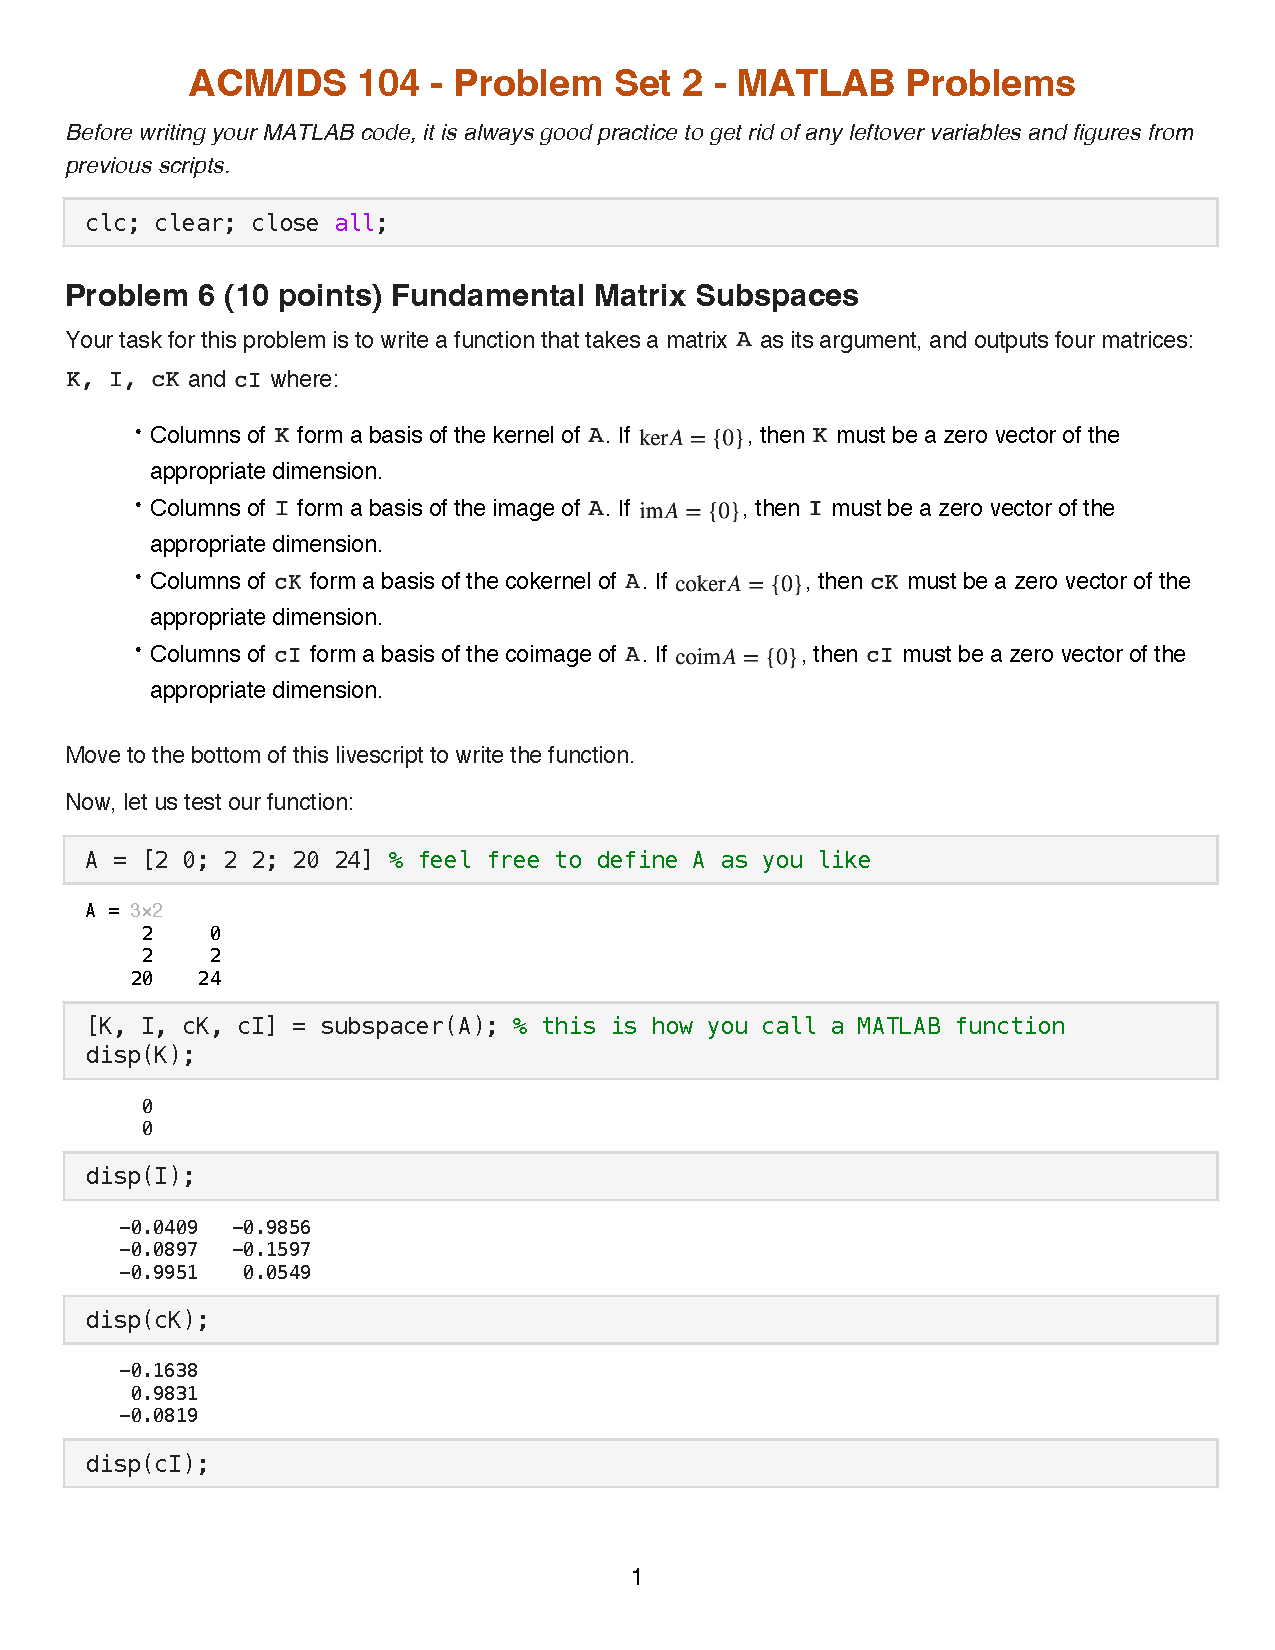
\includepdf[pages=-]{PS2matlab.pdf}



\end{document}
